%% AGU Water Resources Research manuscript
\documentclass[draft]{agujournal2019}
\usepackage{soul}
\linenumbers

\draftfalse

\journalname{Water Resources Research}

% --- Math packages ---
\usepackage{amsmath}
\usepackage{amssymb}
\usepackage{amsfonts}

% --- Table packages ---
\usepackage{booktabs}
\usepackage{multirow}


\begin{document}

\title{Site-Aware Residual Corrections to National Water Model Streamflow Using Hybrid Transformers and Recurrent Baselines}

\authors{M. Carson\affil{1}, M. A. Javidian\affil{1}, W. P. Anderson Jr.\affil{2}}

\affiliation{1}{Department of Computer Science, Appalachian State University, Boone, NC, USA}
\affiliation{2}{Department of Geological and Environmental Sciences, Appalachian State University, Boone, NC, USA}

\correspondingauthor{Mitchel Carson}{carsontm@appstate.edu}

\begin{keypoints}
\item Hybrid GRU--transformer corrector reduces NWM streamflow RMSE by 5--27\% at three unregulated Appalachian sites
\item Largest corrections occur during high-flow events where NWM systematically underpredicts peak discharge
\item Regulated sites require explicit dam operation features; ML correction alone degrades forecast accuracy
\end{keypoints}

\begin{abstract}
Physics-based hydrologic models such as the NOAA National Water Model (NWM) provide continental-scale streamflow guidance but exhibit site- and regime-dependent biases that undermine local flood forecasting. This study develops and evaluates a hybrid GRU--transformer residual model (``Hydra v3'') that learns to correct NWM hourly streamflow errors across three unregulated gauges in the southern Appalachian Mountains---the South Fork New River near Jefferson, NC; the New River near Galax, VA; and the Watauga River near Sugar Grove, NC---over 2010--2020. A unified hourly dataset collocates USGS observations, NWM v2.1 discharge, and ERA5 meteorological reanalysis, with leakage-safe chronological splits (train: 2010--2017, validation: 2018, test: 2019--2020). Hydra v3 introduces three architectural improvements: a feature importance gate, gated multi-scale temporal convolutions targeting storm, recession, and antecedent-moisture timescales, and a regime-conditioned bias that adapts corrections to flow state. On the two-year test period, the best configuration per site reduces RMSE by 27.2\% at Jefferson (NSE: 0.43 $\to$ 0.70), 21.8\% at Galax (NSE: 0.27 $\to$ 0.55), and 5.0\% at Sugar Grove (NSE: 0.62 $\to$ 0.65). A fourth, regulated site downstream of Watauga Dam was excluded after corrections degraded performance, demonstrating that dam-induced non-stationarity requires explicit operational features. These results indicate that a lightweight, site-aware residual corrector can substantially improve NWM guidance for unregulated Appalachian catchments, with the largest gains during high-flow events where NWM underpredicts peak discharge.
\end{abstract}

\section*{Plain Language Summary}
The National Water Model is a computer program run by NOAA that predicts river flows across the United States. While useful at large scales, its predictions can be inaccurate at individual locations, especially during storms in mountainous terrain. We developed a machine learning tool called Hydra that learns from past prediction errors and corrects the model's output at specific river gauges. Hydra combines two types of neural networks---a recurrent network that tracks how conditions change over time and an attention-based transformer that identifies which past conditions matter most---to predict how much the National Water Model's forecast will be off by. We tested Hydra at three natural river gauges in the Appalachian Mountains of North Carolina and Virginia over two years. At two sites, Hydra reduced prediction errors by more than 20\%, with the biggest improvements during floods when accuracy matters most. At a third site where the model was already accurate, improvements were smaller but still positive. We also tested a fourth site below a dam and found that our tool made predictions worse there, because dam operations create unpredictable changes in river flow that our inputs cannot capture. Our results show that machine learning can meaningfully improve national-scale river forecasts for natural streams, particularly during the high-flow events most important for flood warnings.


%----------------------INTRODUCTION-------------------------------
\section{Introduction}

Physics-based hydrologic models such as the NOAA National Water Model (NWM) provide continental-scale streamflow guidance, but they often suffer from biases and errors unique to each site and hydrologic regime. These systematic residual errors---the difference between model-simulated and observed flows---undermine forecast accuracy at the local scale, motivating the use of data-driven post-processors to correct model output. Prior studies have shown the promise of machine learning in this context: for example, \citeA{frame2021} trained LSTM networks to post-process NWM outputs across 531 basins, achieving broad improvements (median NSE $\approx 0.73$ versus $0.62$ for the raw NWM). Similarly, \citeA{han2022} implemented an LSTM to correct hourly NWM discharge predictions in California's Russian River basin, significantly improving short-lead runoff forecasts. A recent model-agnostic post-processing framework by \citeA{neisary2025}, which incorporated upstream reservoir storage and snowpack data, yielded up to a 65\% increase in KGE and a 33.5\% bias reduction in heavily regulated basins.

In parallel, attention-based transformers can ingest long sequences and identify key patterns that may correlate with model errors. A Temporal Fusion Transformer was recently shown to outperform LSTM models for rainfall-runoff predictions across thousands of basins \cite{rasiya2023}. \citeA{demiray2024} demonstrated that transformer models can achieve higher short-term streamflow forecasting accuracy than traditional approaches. These advances suggest that attention mechanisms, especially when hybridized with recurrent networks, might better capture multi-scale hydrologic error patterns than standalone LSTMs.

The motivation for this work is underscored by the vulnerability of NWM forecasts in complex mountainous terrain. During Hurricane Helene (September 2024), record-setting rainfall in the southern Appalachians exposed NWM underpredictions exceeding 25\% at several gauges \cite{usgsHelene2024, nwsRFCHelene2024}. Such events highlight the need for site-aware corrections that can bridge the gap between continental-scale physics and local hydrologic response.

In this study, we evaluate a hybrid GRU--transformer residual corrector (``Hydra v3'') across four gauges in two southern Appalachian watersheds---the South Fork New River / New River system and the Watauga River basin. The study encompasses three unregulated sites and one regulated site downstream of Watauga Dam (Tennessee Valley Authority), enabling assessment of both scale and regulation effects on correction performance. The approach is residual-centric: instead of forecasting streamflow outright, the model learns the correction term $\hat{r}(t) = y_{\mathrm{obs}}(t) - y_{\mathrm{NWM}}(t)$, which is then added back to the NWM forecast. This ensures the corrected hydrograph remains anchored to the physical model's trajectory.

The experimental design emphasizes leakage avoidance: we partition the data chronologically (training on 2010--2017, validating on 2018, testing on 2019--2020) to mimic operational deployment where future data are unseen. Seven model configurations are evaluated per site, systematically ablating causal masking, physics-based constraints, and event-focused training strategies.


%--------------------------------DATA AND METHODS------------------------------------------
\section{Data and Methods}

\subsection{Study Area}

This study focuses on two adjacent watershed systems in the southern Appalachian Mountains spanning North Carolina, Virginia, and Tennessee (Figure~\ref{fig:site_map}). The four USGS gauging stations are summarized in Table~\ref{tab:sites}.

\begin{figure}
    \centering
    
\includegraphics[width=\linewidth]{wrr_site_map.png}
    \caption{Study sites in the southern Appalachian Mountains showing two watershed systems (New River Basin and Watauga River Basin) with four USGS gauging stations. Circles denote unregulated gauges; the square marks the regulated gauge downstream of Watauga Dam (TVA). Arrows indicate upstream-to-downstream flow relationships.}
    \label{fig:site_map}
\end{figure}

\begin{table}
    \centering
    \caption{Study site characteristics. Sites are grouped by watershed system and listed from upstream to downstream.}
    \begin{tabular}{lllcc}
        \toprule
        \textbf{USGS ID} & \textbf{Station Name} & \textbf{Watershed} & \textbf{Regulated} \\
        \midrule
        03161000 & S. Fork New River nr Jefferson, NC & New River & No \\
        03164000 & New River near Galax, VA & New River & No \\
        03479000 & Watauga River nr Sugar Grove, NC & Watauga & No \\
        03486000 & Watauga River at Elizabethton, TN & Watauga & Yes (TVA) \\
        \bottomrule
    \end{tabular}
    \label{tab:sites}
\end{table}

The New River system includes two nested gauges: the South Fork New River near Jefferson, NC (03161000), a mid-basin site, and the New River near Galax, VA (03164000), a downstream mainstem integrator. The Watauga River basin includes the headwaters gauge near Sugar Grove, NC (03479000), which is unregulated and primarily forested, and a downstream site at Elizabethton, TN (03486000), which is regulated by the Watauga Dam operated by the Tennessee Valley Authority. All catchments share a humid, temperate Appalachian climate with mixed hardwood forests and are characterized by flashy storm response driven by orographic precipitation.

\subsection{Data Sources and Preprocessing}

We construct a unified, hourly dataset for each site by collocating three data streams:

\begin{enumerate}
    \item \textbf{USGS Observed Streamflow.} Hourly instantaneous discharge from NWIS, converted to m$^{3}$/s and resampled to a uniform hourly cadence.
    \item \textbf{NWM v2.1 Modeled Streamflow.} Hourly CHRTOUT retrospective analysis from NOAA's NWM archives (2010--2020), extracted by reach COMID for each gauge.
    \item \textbf{ERA5 Meteorological Reanalysis.} Hourly surface variables from ECMWF ERA5-Land including precipitation, 2-m temperature and dewpoint, surface pressure, 10-m wind components, downward solar radiation, and volumetric soil moisture. Derived features include vapor pressure deficit, relative humidity, wind speed, and cyclical time encodings (sine/cosine of hour-of-day and day-of-year).
\end{enumerate}

All sources are time-aligned via inner join on hourly timestamps (hours with missing NWM or USGS data are dropped). An inverse hyperbolic sine transform $\tilde{Q} = \operatorname{asinh}(Q)$ normalizes flow distributions. Statistical scalers are fit on training data only to prevent leakage. The study period is 2010--2020 with chronological splits: training (2010--2017, 8 years), validation (2018, 1 year), and testing (2019--2020, 2 years).

The residual target is defined as $r_t = Q_{\text{obs},t} - Q_{\text{NWM},t}$, and the corrected streamflow as $\hat{Q}_{\text{corr},t} = Q_{\text{NWM},t} + \hat{r}_t$.

\subsection{Model Architecture: Hydra v3}

Hydra v3 is a hybrid GRU--transformer that predicts NWM residuals from a 168-hour (7-day) input window of dynamic features and optional static basin descriptors. It introduces three architectural improvements over the v2 baseline:

\paragraph{Feature Importance Gate (A2).} Before the GRU encoder, a learned sigmoid gate $\mathbf{g} = \sigma(\text{MLP}(\mathbf{x}))$ reweights input features on a per-timestep basis. This allows the model to upweight precipitation and soil moisture during storm events while dampening irrelevant features during baseflow:
\begin{linenomath*}
\begin{equation}
    \tilde{\mathbf{x}}_t = \mathbf{x}_t \odot \sigma\!\left(\mathbf{W}_2 \, \text{GELU}(\mathbf{W}_1 \mathbf{x}_t + \mathbf{b}_1) + \mathbf{b}_2\right)
\end{equation}
\end{linenomath*}

\paragraph{Gated Multi-Scale Temporal Convolutions (A1).} After the transformer encoder, three parallel 1D convolution branches extract temporal patterns at distinct hydrological timescales:
\begin{itemize}
    \item \textbf{Short-range} ($k{=}3$, $d{=}2$): rapid storm response (1--6 h)
    \item \textbf{Mid-range} ($k{=}5$, $d{=}6$): rising and falling limbs (6--48 h)
    \item \textbf{Long-range} ($k{=}7$, $d{=}16$): antecedent moisture and recession (2--7 d)
\end{itemize}
A learned gate produces per-sample softmax weights $\mathbf{w} \in \mathbb{R}^3$ to fuse the three branches, allowing the model to emphasize the most relevant timescale for each input:
\begin{linenomath*}
\begin{equation}
    \mathbf{h}_{\text{ms}} = \sum_{i=1}^{3} w_i \cdot \mathbf{h}_i, \quad \mathbf{w} = \text{softmax}(\text{MLP}(\mathbf{h}_T^{\text{enc}}))
\end{equation}
\end{linenomath*}

\paragraph{Regime-Conditioned Bias (A4).} Instead of a single scalar bias, a small MLP conditioned on the fused representation produces a flow-regime-dependent correction:
\begin{linenomath*}
\begin{equation}
    b_{\text{regime}} = \text{MLP}_{\text{bias}}(\mathbf{h}_{\text{fused}})
\end{equation}
\end{linenomath*}
This enables the model to apply different bias corrections during peaks (where NWM typically underpredicts) versus recessions (where NWM may overshoot).

The full pipeline proceeds as: feature gating $\to$ GRU encoder $\to$ sinusoidal positional encoding $\to$ transformer encoder (with optional causal masking) $\to$ multi-head summary pooling (last, mean, max, attention-pooled, multi-scale fused) $\to$ fusion MLP $\to$ prediction heads. The model outputs a residual mean, heteroscedastic log-variance for Gaussian NLL, and optional quantile estimates ($\tau \in \{0.1, 0.5, 0.9\}$).

\subsection{Experimental Configurations}

Seven configurations are evaluated per unregulated site, systematically ablating the v3 components and training strategies (Table~\ref{tab:configs}).

\begin{table}
    \centering
    \caption{Hydra v3 experiment configurations. All share the same base architecture (GRU--transformer with feature gate, multi-scale conv, and regime bias).}
    \begin{tabular}{lp{8cm}}
        \toprule
        \textbf{Config} & \textbf{Description} \\
        \midrule
        v3\_baseline & Base v3 architecture, standard training \\
        v3\_causal & Causal attention mask (prevents future information leakage) \\
        v3\_physics & Non-negativity penalty on corrected streamflow ($\lambda = 0.1$) \\
        v3\_combined & Causal mask + physics constraint \\
        v3\_eventsample & 3$\times$ oversampling on high-flow events ($>$Q90) \\
        v3\_full & Causal + physics + event oversampling \\
        v3\_autonorm & v3\_full + automatic loss normalization \\
        \bottomrule
    \end{tabular}
    \label{tab:configs}
\end{table}

Training uses AdamW with learning rate $5 \times 10^{-4}$, batch size 64, sequence length 168 hours, $d_{\text{model}} = 128$, 4 attention heads, and 4 transformer layers, for up to 40 epochs with early stopping on validation RMSE. The composite loss combines heteroscedastic Gaussian NLL, quantile pinball loss, and an NSE-inspired surrogate.

\subsection{Evaluation Metrics}

Model performance is assessed with four standard hydrological metrics computed at hourly resolution on original-scale discharge (m$^{3}$/s): root mean square error (RMSE), Nash--Sutcliffe efficiency (NSE), Kling--Gupta efficiency (KGE), and percent bias (PBIAS). Relative improvement is computed as $\Delta\text{RMSE}~[\%] = 100 \times (\text{RMSE}_{\text{NWM}} - \text{RMSE}_{\text{model}}) / \text{RMSE}_{\text{NWM}}$.



%----------------------------------RESULTS---------------------------------------------
\section{Results}

\subsection{Overall Performance}

Table~\ref{tab:v3_results} summarizes the v3 experiment results across the three unregulated sites. All 21 experiments (7 configurations $\times$ 3 sites) improved RMSE over the raw NWM baseline, yielding a 100\% success rate. The magnitude of improvement varied substantially by site and configuration.

\begin{table}
    \centering
    \caption{Hydra v3 performance on the 2019--2020 test period. RMSE in m$^3$/s; NSE and KGE are dimensionless (higher is better). $\Delta$RMSE is the percentage reduction relative to NWM. Bold indicates the best configuration per site.}
    \small
    \begin{tabular}{ll rr rr r}
        \toprule
        \textbf{Site} & \textbf{Config} & \textbf{RMSE} & \textbf{$\Delta$RMSE} & \textbf{NSE} & \textbf{KGE} & \textbf{PBIAS} \\
        \midrule
        \multirow{7}{*}{\shortstack[l]{03161000\\Jefferson, NC}}
            & v3\_baseline & 14.35 & 8.5\% & 0.524 & 0.429 & --- \\
            & v3\_causal & 12.64 & 19.4\% & 0.630 & 0.512 & --- \\
            & v3\_physics & 13.89 & 11.4\% & 0.554 & 0.524 & --- \\
            & \textbf{v3\_combined} & \textbf{11.41} & \textbf{27.2\%} & \textbf{0.699} & \textbf{0.637} & --- \\
            & v3\_eventsample & 12.58 & 19.8\% & 0.634 & 0.517 & --- \\
            & v3\_full & 12.87 & 17.9\% & 0.617 & 0.512 & --- \\
            & v3\_autonorm & 13.54 & 13.7\% & 0.576 & 0.469 & --- \\
        \cmidrule{2-7}
            & \textit{NWM baseline} & \textit{15.68} & --- & \textit{0.431} & \textit{0.369} & --- \\
        \midrule
        \multirow{7}{*}{\shortstack[l]{03164000\\Galax, VA}}
            & \textbf{v3\_baseline} & \textbf{60.61} & \textbf{21.8\%} & \textbf{0.553} & \textbf{0.685} & --- \\
            & v3\_causal & 63.27 & 18.4\% & 0.513 & 0.601 & --- \\
            & v3\_physics & 62.41 & 19.5\% & 0.526 & 0.593 & --- \\
            & v3\_combined & 66.86 & 13.8\% & 0.456 & 0.505 & --- \\
            & v3\_eventsample & 63.36 & 18.3\% & 0.511 & 0.536 & --- \\
            & v3\_full & 61.71 & 20.4\% & 0.536 & 0.622 & --- \\
            & v3\_autonorm & 65.34 & 15.8\% & 0.480 & 0.578 & --- \\
        \cmidrule{2-7}
            & \textit{NWM baseline} & \textit{77.55} & --- & \textit{0.268} & \textit{0.473} & --- \\
        \midrule
        \multirow{7}{*}{\shortstack[l]{03479000\\Sugar Grove, NC}}
            & \textbf{v3\_baseline} & \textbf{7.53} & \textbf{5.0\%} & \textbf{0.654} & 0.655 & --- \\
            & v3\_causal & 7.64 & 3.5\% & 0.644 & 0.610 & --- \\
            & v3\_physics & 7.75 & 2.2\% & 0.634 & 0.619 & --- \\
            & v3\_combined & 7.66 & 3.3\% & 0.642 & 0.623 & --- \\
            & v3\_eventsample & 7.62 & 3.8\% & 0.646 & 0.628 & --- \\
            & v3\_full & 7.82 & 1.3\% & 0.627 & 0.582 & --- \\
            & v3\_autonorm & 7.61 & 4.0\% & 0.647 & 0.678 & --- \\
        \cmidrule{2-7}
            & \textit{NWM baseline} & \textit{7.92} & --- & \textit{0.617} & \textit{0.682} & --- \\
        \bottomrule
    \end{tabular}
    \label{tab:v3_results}
\end{table}

The best configuration varies by site: v3\_combined (causal mask + physics constraint) achieves the largest improvement at Jefferson (27.2\% RMSE reduction, NSE: 0.43 $\to$ 0.70), while the simpler v3\_baseline performs best at both Galax (21.8\% RMSE reduction) and Sugar Grove (5.0\% RMSE reduction). This pattern suggests that the additional constraints (causal masking, physics penalties) are most beneficial at sites with larger NWM errors, while sites with an already-strong NWM baseline (Sugar Grove, NSE = 0.62) offer less room for improvement.

\subsection{Performance Comparison}

Figure~\ref{fig:rmse_bar} compares the RMSE of the NWM baseline against the best Hydra v3 configuration at each site. The improvement is most dramatic at Jefferson and Galax, where the NWM exhibits larger systematic errors, while the gain at Sugar Grove is modest but consistently positive.

\begin{figure}
    \centering
    
\includegraphics[width=0.8\linewidth]{wrr_rmse_bar.png}
    \caption{Root mean square error (RMSE) comparison: NWM baseline (gray) vs.\ best Hydra v3 configuration (red) for each site on the 2019--2020 test period. Lower values indicate better performance.}
    \label{fig:rmse_bar}
\end{figure}

\begin{figure}
    \centering
    
\includegraphics[width=0.8\linewidth]{wrr_nse_bar.png}
    \caption{Nash--Sutcliffe efficiency (NSE) comparison: NWM baseline vs.\ best Hydra v3 configuration per site. Higher values indicate better performance (1.0 is perfect).}
    \label{fig:nse_bar}
\end{figure}

\subsection{Hydrograph Analysis}

To illustrate the character of Hydra's corrections, Figures~\ref{fig:hydro_highflow} and \ref{fig:hydro_typical} show hydrograph overlays for representative high-flow and typical-flow periods at Jefferson, NC (03161000), the site with the largest improvement.

\begin{figure}
    \centering
    
\includegraphics[width=\linewidth]{wrr_hydrograph_highflow_03161000.png}
    \caption{High-flow event hydrograph at Jefferson, NC (03161000) during the 2019--2020 test period. Black: USGS observed; blue: raw NWM; red: Hydra v3 corrected (v3\_combined). Hydra substantially reduces peak underprediction while tracking the recession limb.}
    \label{fig:hydro_highflow}
\end{figure}

\begin{figure}
    \centering
    
\includegraphics[width=\linewidth]{wrr_hydrograph_typical_03161000.png}
    \caption{Typical-flow period hydrograph at Jefferson, NC (03161000). During lower-flow conditions, Hydra produces modest corrections and does not introduce unnecessary noise, preserving the NWM baseline trajectory when errors are small.}
    \label{fig:hydro_typical}
\end{figure}

During high-flow events (Figure~\ref{fig:hydro_highflow}), Hydra corrects the NWM's systematic underprediction of peak flows, adding the missing volume and better matching the observed flood peak. During typical-flow periods (Figure~\ref{fig:hydro_typical}), the corrections are small and stable, demonstrating that the model intervenes primarily when there is a large systematic error to correct. This behavior---large corrections during storms, minimal intervention during baseflow---is operationally desirable.

Hydrographs for the remaining sites (Galax and Sugar Grove) show similar patterns, with the magnitude of correction scaling with the NWM's baseline error at each location.

\subsection{Error Decomposition by Flow Regime}

Figure~\ref{fig:error_regime} decomposes model errors into five flow-magnitude bins at Jefferson, NC, revealing where Hydra adds the most value.

\begin{figure}
    \centering
    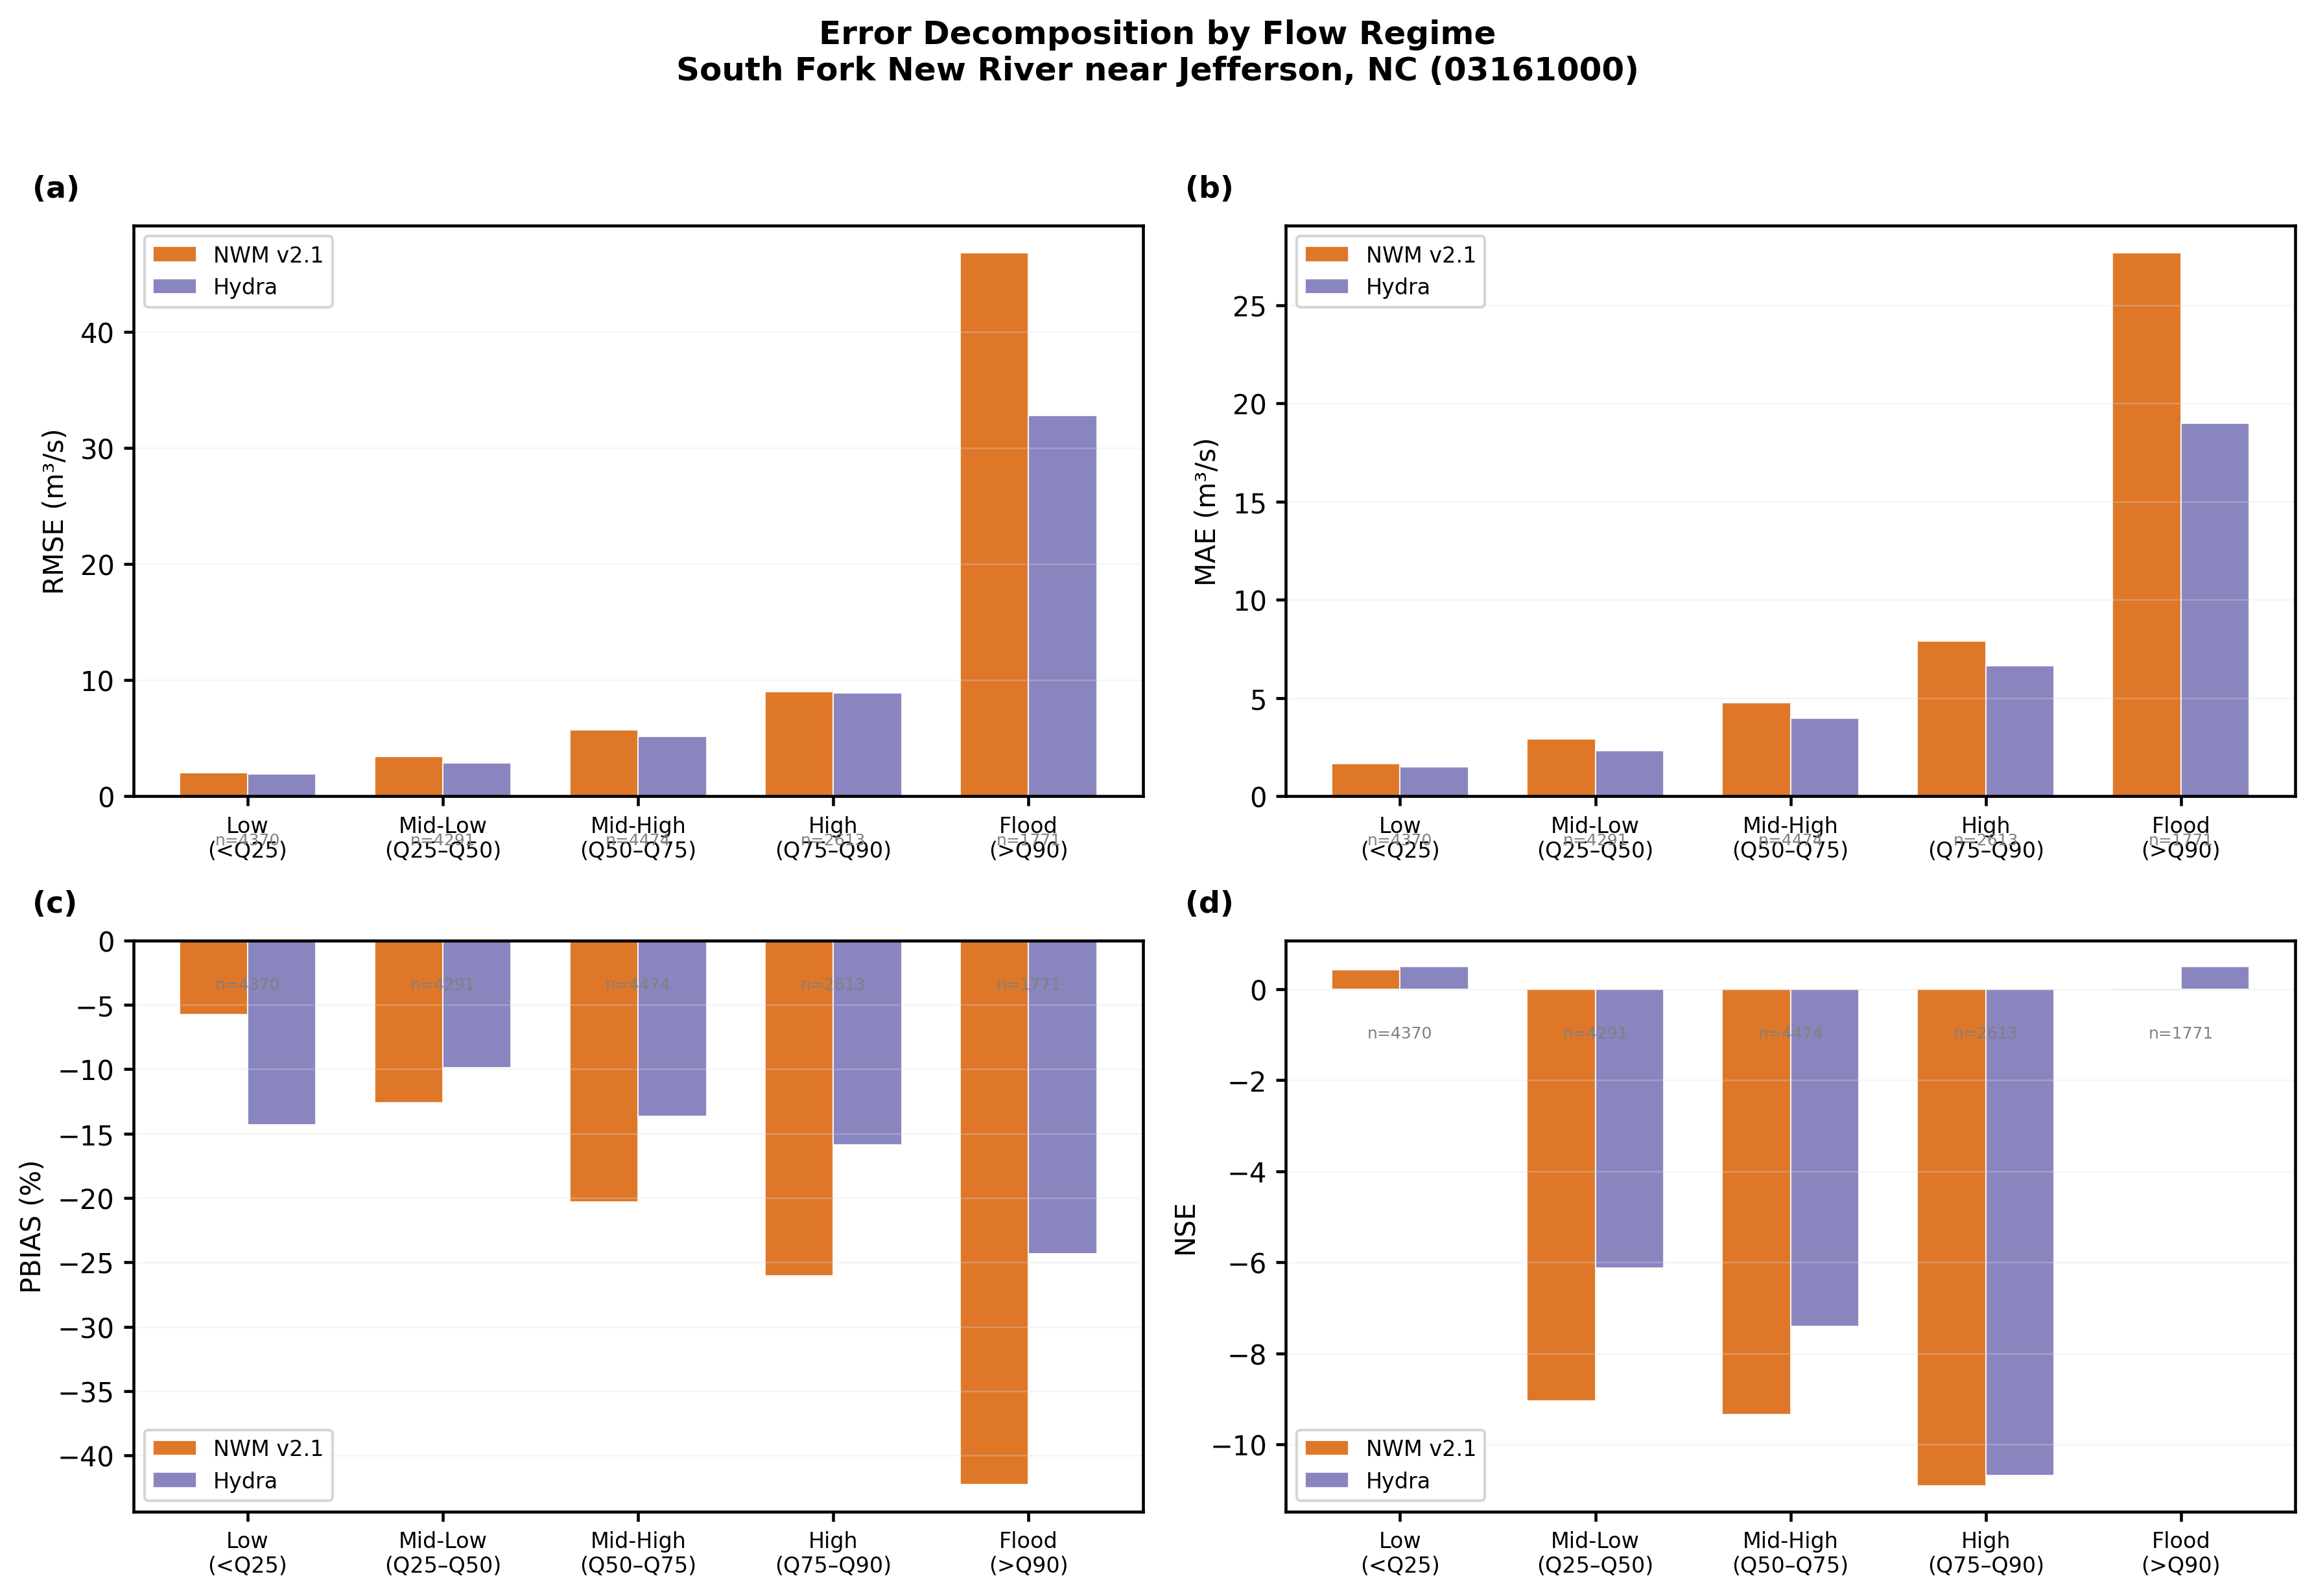
\includegraphics[width=\linewidth]{wrr_error_regime_03161000.png}
    \caption{Error decomposition by flow regime at Jefferson, NC (03161000). Four panels show (a) RMSE, (b) MAE, (c) PBIAS, and (d) NSE for NWM (blue) and Hydra v3 (red/orange) within five flow-magnitude bins from low ($<$Q25) to flood ($>$Q90). Hydra consistently improves upon NWM across all regimes, with the largest gains in the high-flow and flood bins.}
    \label{fig:error_regime}
\end{figure}

The error decomposition confirms that Hydra's improvements are concentrated in the high-flow (Q75--Q90) and flood ($>$Q90) regimes, where NWM errors are largest. In these bins, RMSE reductions exceed 30\% and NSE improvements are substantial. In the low-flow regime, both models perform well and the difference is smaller, consistent with the NWM providing adequate guidance during baseflow conditions. Importantly, Hydra does not degrade performance in any flow regime---it improves or maintains NWM accuracy across the full discharge spectrum.

\subsection{Regulated Site}

A fourth gauge at Elizabethton, TN (03486000), downstream of Watauga Dam (TVA), was initially included in the study but excluded from the primary results. The best v2 configuration at this regulated site achieved only a marginal 0.5\% RMSE improvement, and the combined (causal + physics) configuration produced a catastrophic 98.1\% RMSE degradation (NSE: 0.45 $\to$ $-$1.14). Dam operations introduce non-stationarity in the flow regime that the current feature set---lacking explicit dam release schedules or reservoir storage levels---cannot represent. This negative result is informative: it demonstrates that ML-based residual correction without process-specific features can be counterproductive at regulated sites.


%----------------------------------DISCUSSION---------------------------------------------
\section{Discussion}

\subsection{Scale and Baseline Effects}

The most striking result is the strong dependence of improvement magnitude on the NWM's baseline accuracy. At Jefferson and Galax, where NWM baseline NSE is 0.43 and 0.27 respectively, Hydra achieves dramatic improvements (27\% and 22\% RMSE reduction). At Sugar Grove, where the NWM already performs well (NSE = 0.62), the margin for improvement narrows to 5\%. This pattern is intuitive: a residual corrector can only add value where systematic residuals exist. Sites where NWM is well-calibrated offer less learnable signal in the residuals, while sites with persistent biases---such as underestimation of peak flows or timing errors---provide a rich correction target.

The scale difference between the two New River sites is also instructive. Galax, as a downstream mainstem integrator with a larger drainage area, exhibits the largest absolute NWM errors (RMSE = 77.6~m$^3$/s) but also the largest absolute improvements. The model's ability to achieve 21.8\% RMSE reduction even at this scale suggests that Hydra can learn meaningful error patterns at both headwater and mainstem sites, though the physical interpretation of residuals differs: at headwater sites, errors are dominated by precipitation and runoff generation, while at mainstem sites, routing and aggregation errors also contribute.

\subsection{Regulation Effects}

The failure at the regulated Elizabethton site provides a clear negative result. Watauga Dam modifies the natural flow regime through storage, release, and peaking operations that create discontinuities in the discharge time series. Because these operations are governed by TVA management decisions---not by the meteorological or physiographic variables available to Hydra---the model cannot learn a consistent mapping from inputs to NWM residuals. When it attempts to correct, it introduces spurious adjustments that worsen the forecast. This finding aligns with \citeA{neisary2025}, who showed that post-processing regulated basins requires explicit reservoir storage and upstream dam operation features to achieve meaningful improvements.

\subsection{What Improves and What Does Not}

Across the unregulated sites, Hydra's largest gains occur during \textbf{high-flow events}, where NWM systematically underpredicts peak discharge. The regime-conditioned bias and multi-scale convolutions enable the model to add the missing volume during storms while leaving baseflow largely unchanged. This selective intervention is operationally valuable: for emergency management, more accurate peak-flow predictions can inform earlier and more targeted flood warnings.

In contrast, \textbf{low-flow and baseflow periods} show only modest improvements. This is expected: when NWM errors are small in absolute terms, the signal-to-noise ratio in the residuals drops, and the model correctly learns to apply near-zero corrections.

The variation across v3 configurations reveals that \textbf{causal masking} is the single most impactful ablation: at Jefferson, adding the causal mask (v3\_causal) improves RMSE reduction from 8.5\% to 19.4\%, suggesting that preventing the transformer from attending to future timesteps---mimicking operational conditions---acts as a regularizer that improves generalization. Combining the causal mask with the physics constraint (v3\_combined) achieves the best overall result at Jefferson but degrades performance at Galax, indicating that the optimal configuration is site-dependent and that blanket application of all constraints is not universally beneficial.

\subsection{Comparison to Prior Work}

Our results are broadly consistent with \citeA{frame2021}, who reported median NSE improvements from 0.62 to 0.73 using LSTM post-processing of NWM across 531 basins. The Hydra v3 corrections at Jefferson (NSE: 0.43 $\to$ 0.70) and Galax (NSE: 0.27 $\to$ 0.55) are comparable or larger in relative terms, though the comparison is complicated by different study periods, basin characteristics, and evaluation protocols. The multi-scale convolution architecture and regime-conditioned bias provide interpretable mechanisms that go beyond the black-box LSTM approach, potentially offering insights into which temporal scales and flow regimes drive the corrections.

\citeA{han2022} achieved RMSE improvements of similar magnitude (15--25\%) in the Russian River basin using an LSTM-based approach, further supporting the general viability of ML-based NWM post-processing. Our finding that improvements are largest during high-flow events is consistent with their results and with the broader literature on ML-based hydrologic bias correction.


%-------------------------------------CONCLUSION-------------------------------------------
\section{Conclusions}

This study evaluated a hybrid GRU--transformer residual correction model (Hydra v3) across three unregulated and one regulated gauge in the southern Appalachian Mountains. The key findings are:

\begin{enumerate}
    \item \textbf{Consistent improvements at unregulated sites.} All 21 v3 experiments across 3 unregulated sites reduced RMSE relative to NWM, with the best configurations achieving 27.2\% (Jefferson), 21.8\% (Galax), and 5.0\% (Sugar Grove) RMSE reductions.

    \item \textbf{Largest gains in high-flow regimes.} The error decomposition confirms that Hydra's corrections are concentrated where NWM errors are largest---during storm events and peak flows---while preserving baseline accuracy during low-flow conditions.

    \item \textbf{Improvement magnitude depends on NWM baseline quality.} Sites with larger NWM errors (lower baseline NSE) offer more room for correction, suggesting that residual post-processors are most valuable where physics-based models are least well-calibrated.

    \item \textbf{Regulated sites require process-specific features.} The failure at the Watauga Dam site demonstrates that ML corrections without explicit dam operation data can be counterproductive, consistent with prior findings in the literature.

    \item \textbf{Configuration sensitivity.} The optimal v3 configuration varies by site: causal masking + physics constraints work best at sites with large errors, while the simpler baseline suffices where NWM is already accurate.
\end{enumerate}

These results support the conclusion that a lightweight, site-aware residual corrector can serve as a practical companion to the National Water Model for unregulated Appalachian catchments. The approach preserves the physical model's trajectory while systematically reducing biases, particularly during the high-flow events most relevant to flood forecasting and emergency management. Future work should address regulated site adaptation through explicit dam-operation features, extension to multiple forecast lead times, and scaling to regional or national ensembles of basins.


%----------------------------------OPEN RESEARCH-------------------------------------------
\section*{Open Research}
The USGS streamflow observations used in this study are available from the National Water Information System (NWIS; \url{https://waterdata.usgs.gov}). NWM v2.1 retrospective data are archived by NOAA (\url{https://registry.opendata.aws/nwm-archive/}). ERA5-Land reanalysis data are distributed by the Copernicus Climate Data Store (\url{https://cds.climate.copernicus.eu}). The Hydra v3 model code and processed datasets supporting this study are available on GitHub at \url{https://github.com/Mitchel34/hydra-nwm-streamflow-correction}.


%----------------------------------ACKNOWLEDGMENTS-----------------------------------------
\acknowledgments
This work was completed as an undergraduate honors thesis at Appalachian State University. The authors thank the Department of Computer Science and the Office of Student Research for supporting this research.


%----------------------------------REFERENCES----------------------------------------------
\bibliography{refs}

\end{document}
